\documentclass[a4paper, titlepage, oneside, 12pt]{article}%      autres choix : book  report

\usepackage[utf8]{inputenc}%           gestion des accents (source)
\usepackage[T1]{fontenc}%              gestion des accents (PDF)
\usepackage[francais]{babel}%          gestion du français
\usepackage{textcomp}%                 caractères additionnels
\usepackage{mathtools,  amssymb, amsthm}% packages de l'AMS + mathtools
\usepackage{lmodern}%                  police de caractère
\usepackage{geometry}%                 gestion des marges
\usepackage{graphicx}%                 gestion des images
\usepackage{xcolor}%                   gestion des couleurs
\usepackage{array}%                    gestion améliorée des tableaux
\usepackage{calc}%                     syntaxe naturelle pour les calculs
\usepackage{titlesec}%                 pour les sections
\usepackage{titletoc}%                 pour la table des matières
\usepackage{fancyhdr}%                 pour les en-têtes
\usepackage{titling}%                  pour le titre
\usepackage[framemethod=TikZ]{mdframed}% print frames
\usepackage{caption}%                  for captionof
\usepackage{listingsutf8}

\usepackage{enumitem}%                 pour les listes numérotées
\usepackage{microtype}%                améliorations typographiques
\usepackage{csvsimple}%                 convertir un fichier .csv en tableau


\usepackage{hyperref}%                 gestion des hyperliens

\usepackage{titling} %  				  gestion des subtitles 
\newcommand{\subtitle}[1]{%			  definition d'une nouvelle commande sous-titre
  \posttitle{%
    \par\end{center}
    \begin{center}\large#1\end{center}
    \vskip0.5em}%
}                
\lstset{language=c++}
\definecolor{codegreen}{rgb}{0,0.6,0}
\definecolor{codegray}{rgb}{0.5,0.5,0.5}
\definecolor{codepurple}{rgb}{0.58,0,0.82}
\definecolor{backcolour}{rgb}{0.95,0.95,0.92}
 
\lstdefinestyle{mystyle}{
    backgroundcolor=\color{backcolour},   
    commentstyle=\color{codegreen},
    keywordstyle=\color{magenta},
    numberstyle=\tiny\color{codegray},
    stringstyle=\color{codepurple},
    basicstyle=\footnotesize,
    breakatwhitespace=false,         
    breaklines=true,                 
    captionpos=b,                    
    keepspaces=true,                 
    numbers=left,                    
    numbersep=5pt,
    otherkeywords={uint16_t},                  
    showspaces=false,                
    showstringspaces=false,
    inputencoding=latin1,
    showtabs=false,                  
    tabsize=2
}
\lstset{style=mystyle}

\hypersetup{%
    pdfborder = {0 0 0}
}

                                    
\title{Projet PERI :\\ Dispositif météorologique}
\subtitle{Rapport de projet}

\author{ Paul MABILLOT \& Adrien FERREIRA \& Pierre MAHÉ}
\date{\today}


\begin{document} 

\begin{figure}[h]
\maketitle 
\end{figure}

\begin{figure}[b]
	
\includegraphics[width=100px] {upmc_logo.jpg}
\end{figure}

\newpage   
   
\tableofcontents

\newpage

\section{Description du projet}
\section{Montage}
\subsection{Arduino}

\paragraph{}
Faire le montage suivant votre carte Arduino. \\ 
Pour les cartes Nano et One les branchements sont similaire. À noter que nous n'utilisons pas de led externe mais celle intégrée au circuit.
\newline
\\
	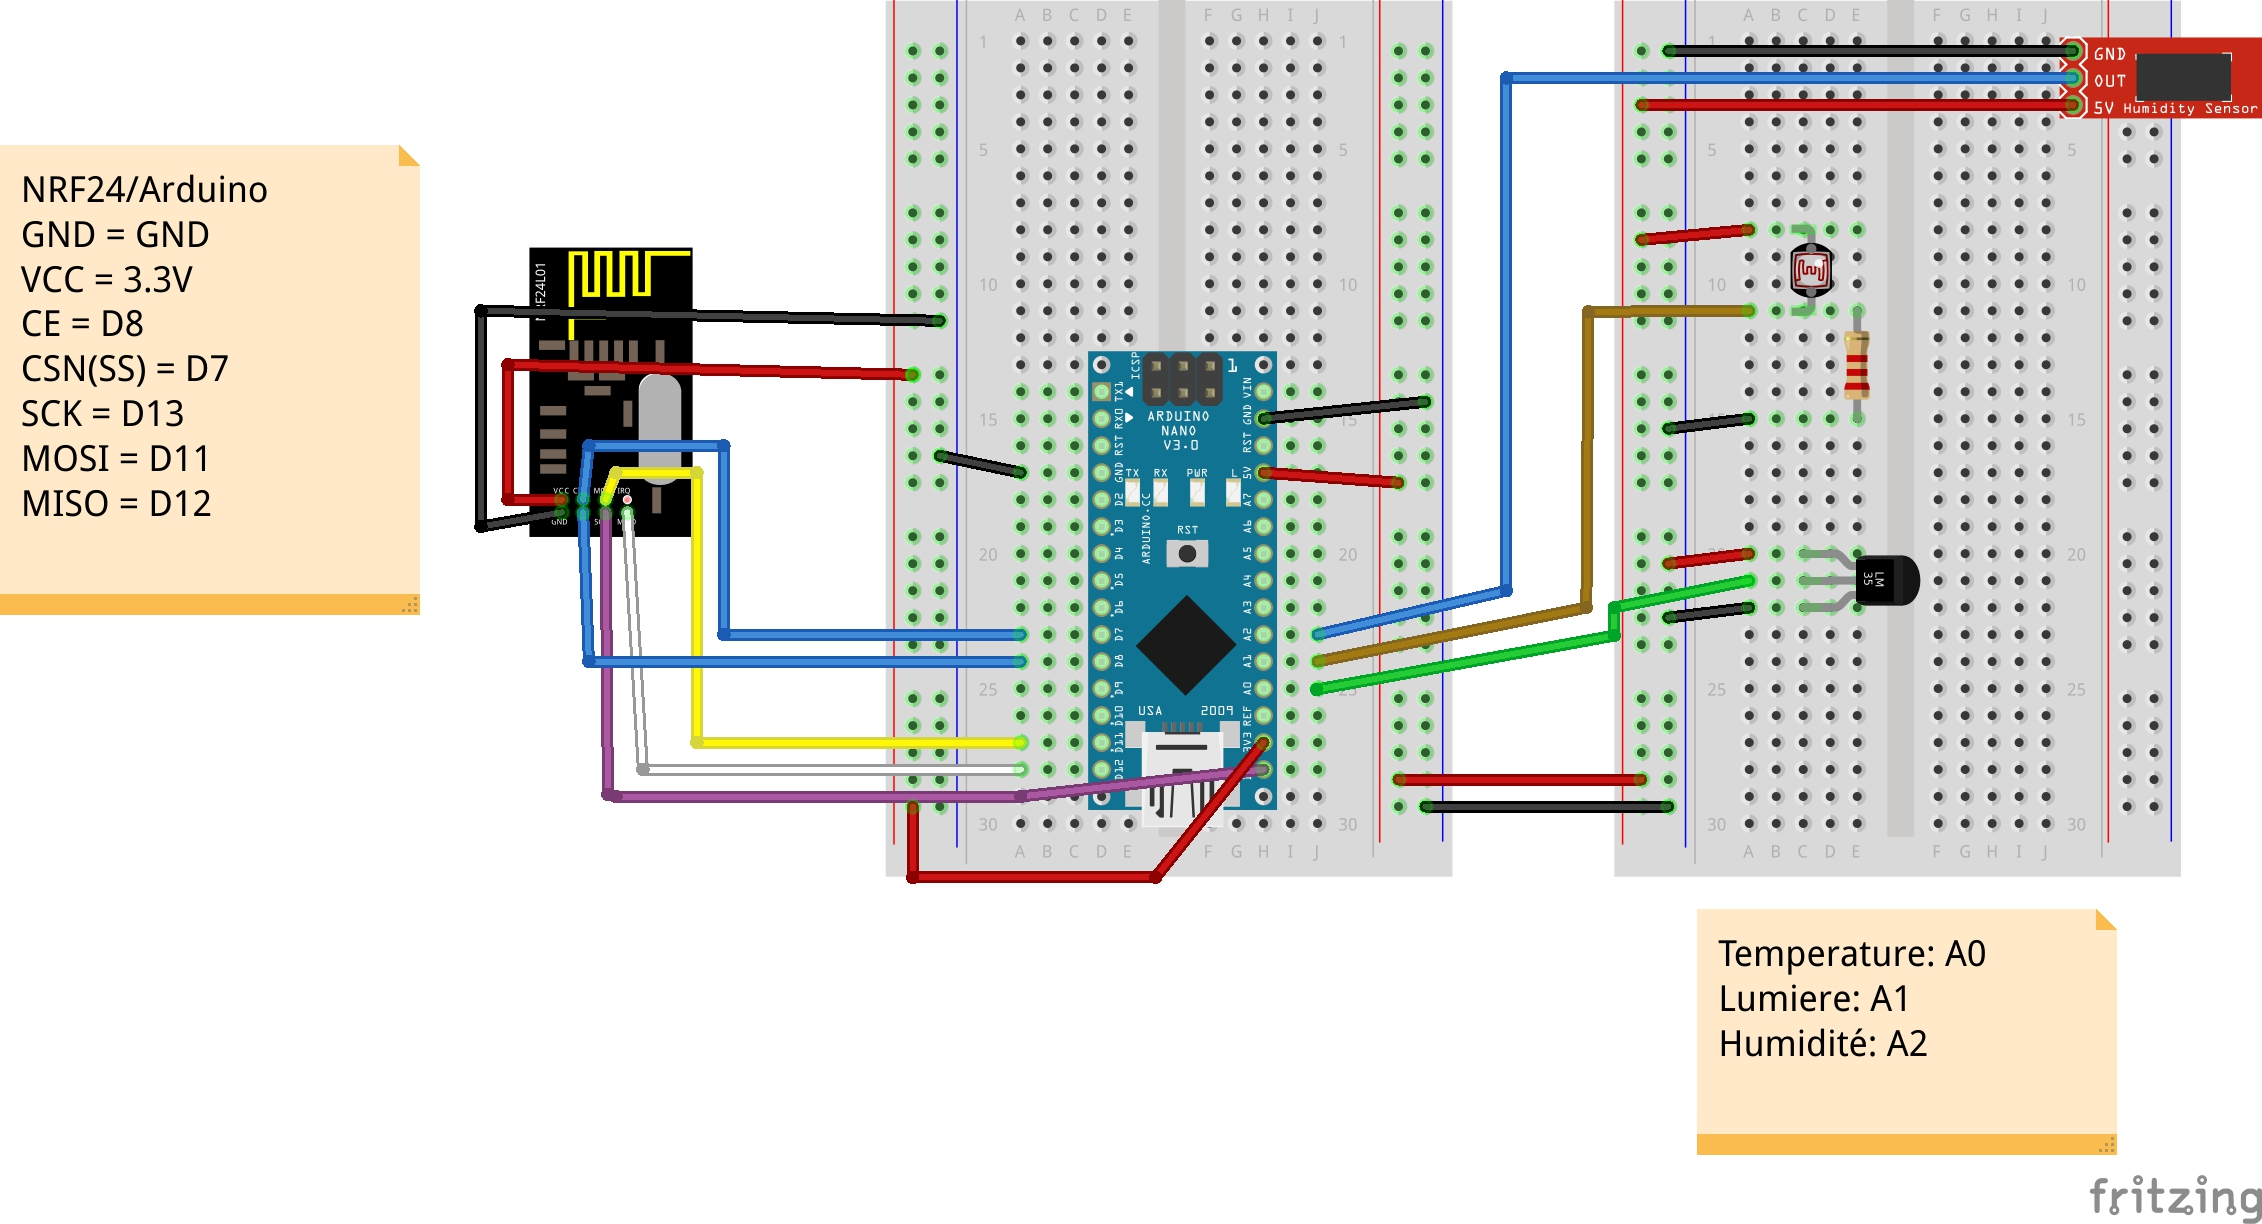
\includegraphics[width=400px] {montage-arduino-nrF24.jpg}

\paragraph{}
Pour l'Arduino Méga le montage est un peu différent.
Branchez le pin CSN(SS) au pin D53, le SCK au pin D52, le MOSI au pin D51 et le MISO au pin D50.
\newline
\\
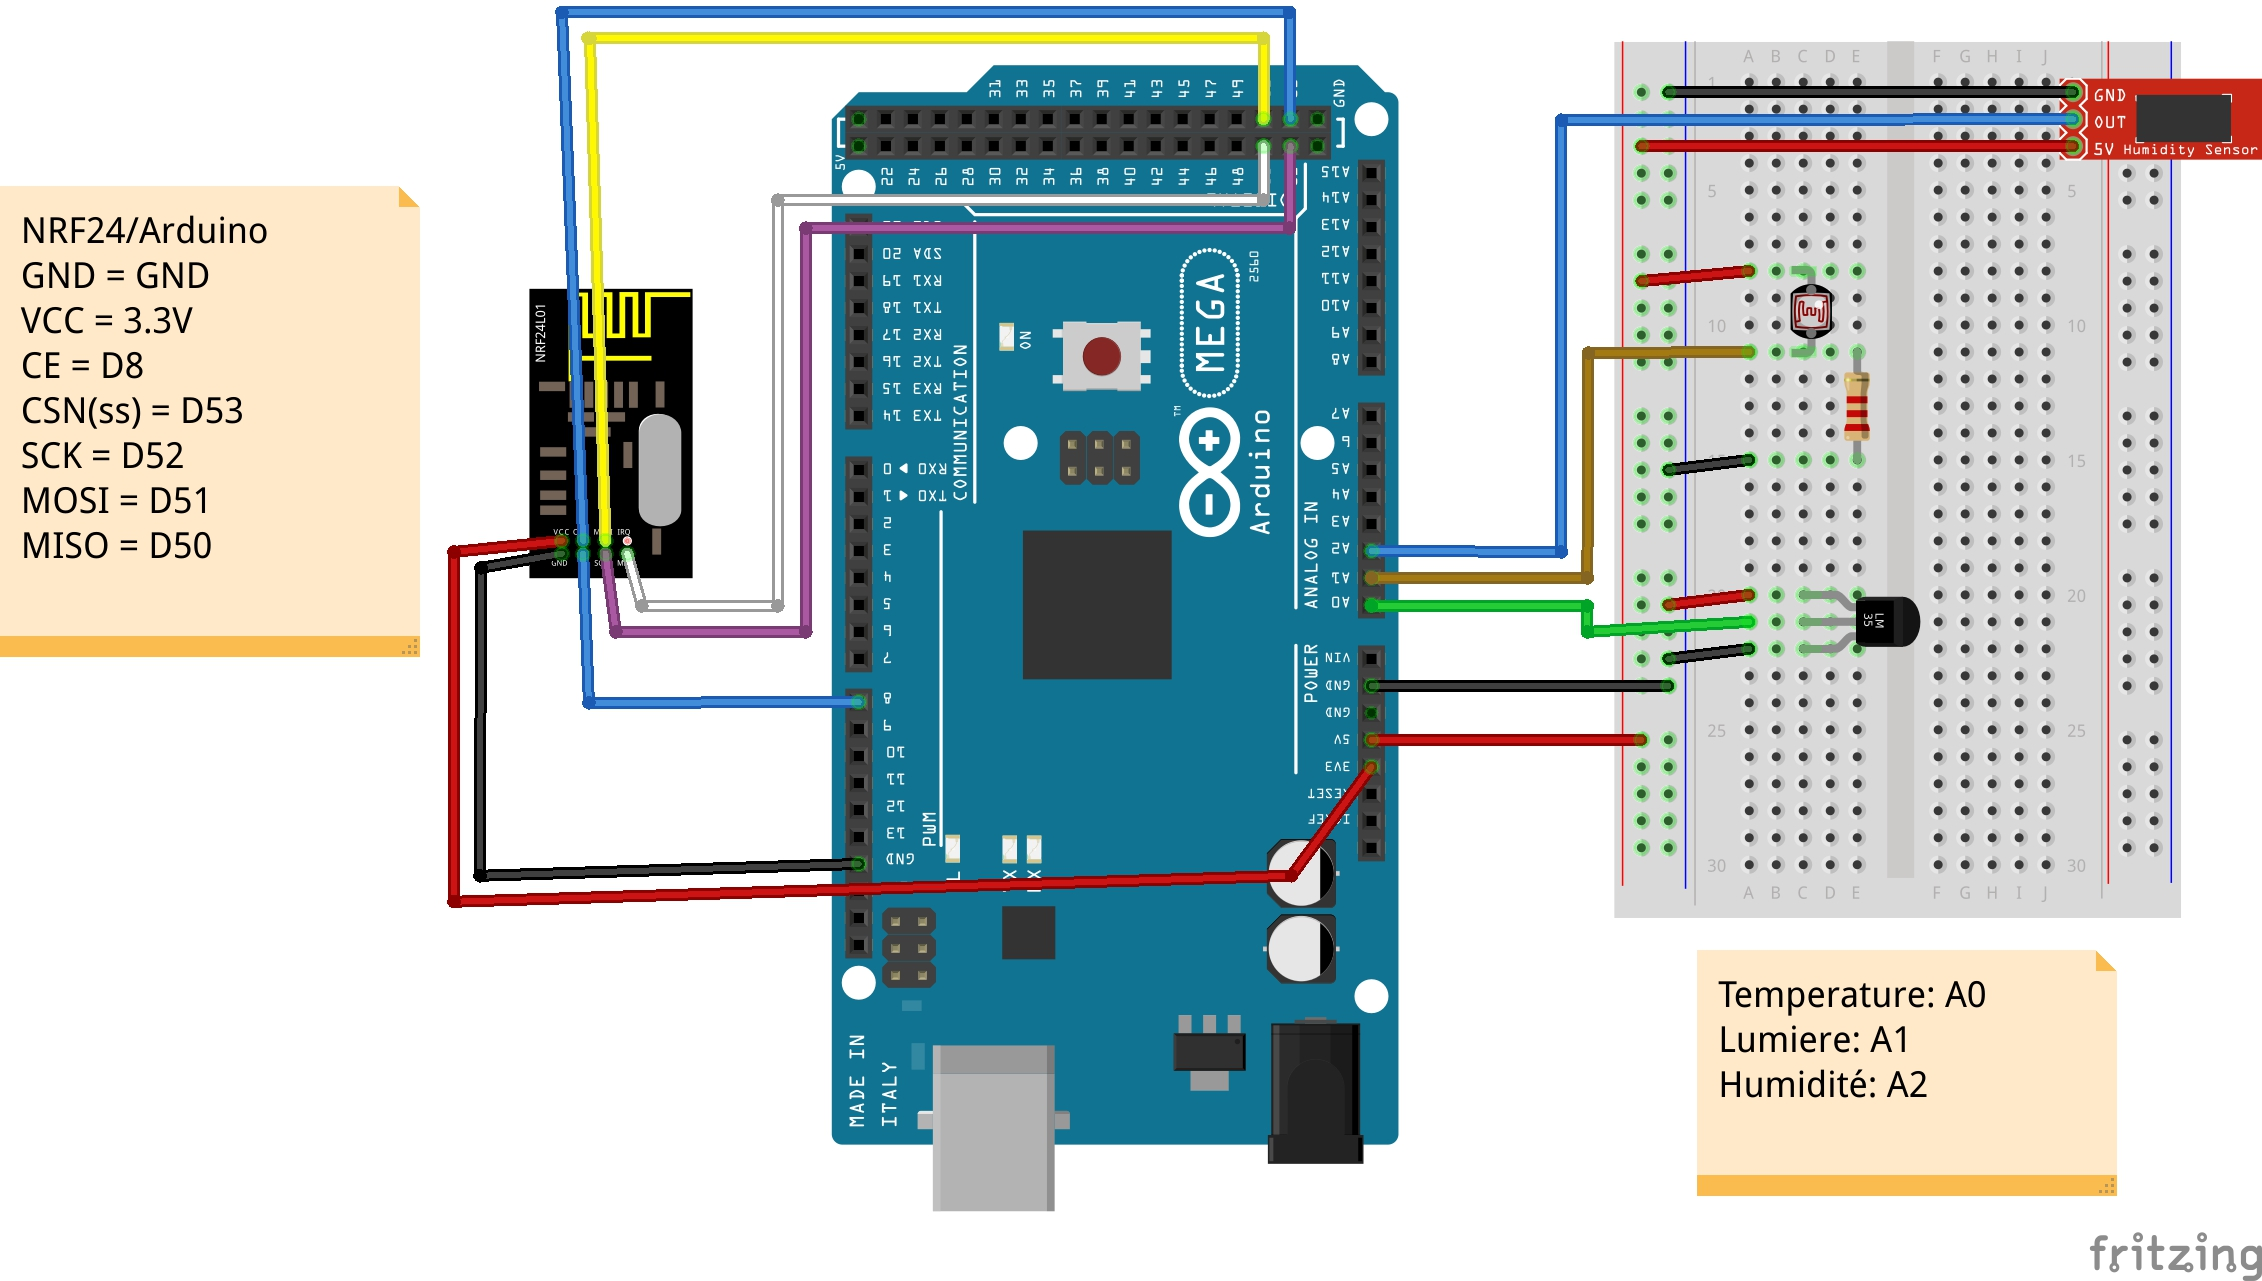
\includegraphics[width=400px] {montage-arduino-mega-nrF24.jpg}

\subsection{Raspberry Pi}
\paragraph{}
Faire le montage suivant sur votre carte Raspberry Pi.\\ Dans cet exemple, nous avons utilisé une Raspberry Pi modèle B mais pour les modèles B+ et 2 la rétrocompatibilité est assurée, il suffit de procéder au même branchement que le schéma.
\newline
\\
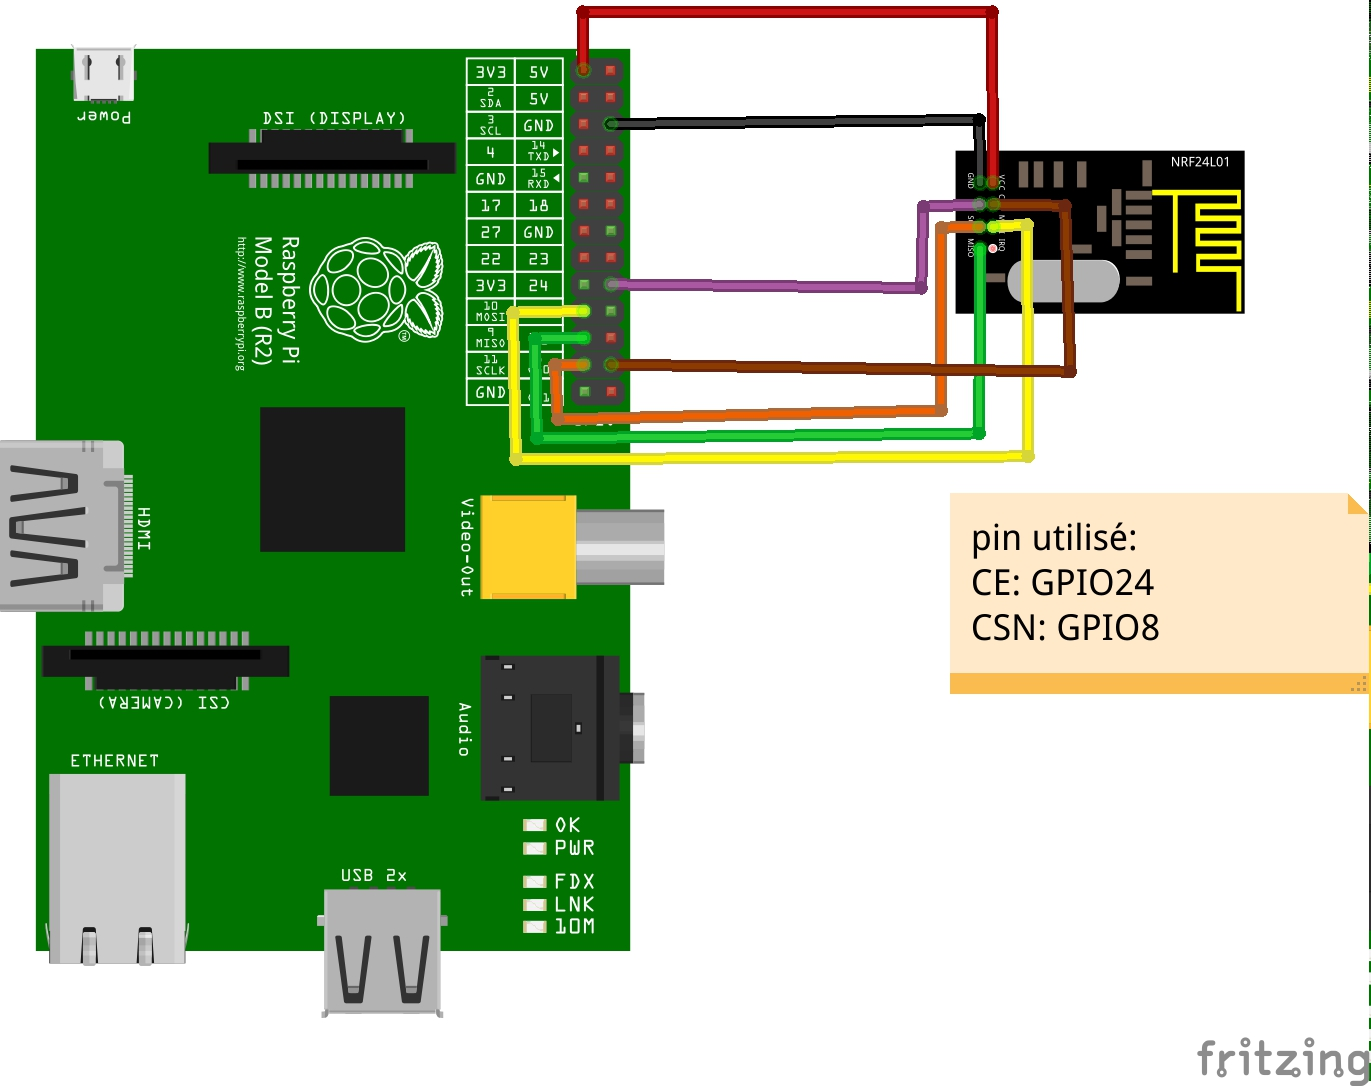
\includegraphics[width=400px] {montage-raspberry-nrF24.jpg}

\paragraph{}
\textbf{Attention: Le module nRF24 est fragile, il n'accepte qu'une alimentation 3.3V, ne surtout pas le brancher sur le pin 5V au risque de l'endommager.}

\section{Codage}
\subsection{Structure de données}
Cette structure est commune aux deux cartes, elle permet de structurer les données envoyées.
\begin{lstlisting}
typedef struct t_payload{
	uint16_t cmd;
	uint16_t timeStamp;
	uint16_t valLight;
	uint16_t valTemperature;
	uint16_t valHumidity;
} payload;
\end{lstlisting}
%TODO changer t_payload
Pour garantir l’interopérabilité, il est impératif de définir explicitement la taille des types manipulés.
\textbf{Attention: certains compilateurs rajoutent des octets de bourrage pour aligner la taille de la structure en mémoire. Veillez donc à accorder les options des deux compilateurs (Arduino et Raspberry).}
L'option \texttt{packed} peut être utilisée comme directive pour le compilateur.
  
L'endianess de l'Arduino et la Raspberry étant identique il n'a pas été nécessaire d'opérer à des conversions, attention cependant au portage sur d'autres systèmes.
\texttt{cmd} utile pour définir le type de traitement à réaliser (cf: Protocole).
Les autres champs sont présents pour stocker les données à proprement parler.
\subsection{Arduino}
\paragraph{}
Pour envoyer les données à intervalle régulière, vous devez installer la bibliothèque \href{http://playground.arduino.cc/Code/SimpleTimer?ref=driverlayer.com/web}{\textit{SimpleTimer}} (téléchargeable sur le site officiel Arduino).\\
Il faut tout d'abord armer un timer avec un temps (en milliseconde) et un pointeur de fonction (sans paramètre) dans le \texttt{setup}. Dans le \texttt{loop}, appelez la fonction \texttt{run}.\\
\begin{lstlisting}
SimpleTimer timer;
timer.setInterval(DELAY, fctnCallback);
timer.run()
\end{lstlisting}


\paragraph{}
Pour communiquer avec le module nRF24L01+, vous devez installer une seconde bibliothèque.
\href{https://github.com/stanleyseow/RF24}{\textit{lien du dépôt}}. Seul les fichiers \texttt{RF24.cpp} et \texttt{RF24.h} sont à copier dans le dossier \texttt{librairies} de l'IDE sketch.
\\ \\
\subsubsection{Initialisation}
La séquence d'instruction à utiliser pour initialiser le module nRF24 est:\\

\begin{lstlisting}
radio.begin();
radio.setPALevel(RF24_PA_MAX);	// la force d'émission du signal
radio.setDataRate(RF24_1MBPS);	// le débit de données

// Identifiant arbitraire du canal de émission 
radio.openWritingPipe(0x0000000001LL);
// Identifiant du canal de réception pour le pipe 1
radio.openReadingPipe(1, 0x0000000002LL);
\end{lstlisting}
\paragraph{}
\textbf{Attention: Il n'est possible d’écouter que sur 6 canaux simultanément.\\}
Attention à correctement synchroniser les canaux utilisés par les nœuds. Si deux modules écrivent sur le même canal, des collisions vont apparaître.

\subsubsection{Lecture}
Avant de pouvoir envoyer des données grâce au module nRF24, il faut l'activer en lecture grâce à l'instruction : \texttt{startListening()}.
Pour savoir si une donnée est en attente dans le buffer de réception, il faut utiliser l'instruction \texttt{available()} non-bloquante.
Pour récupérer la valeur, il faut utiliser \texttt{read}.

\subsubsection{Écriture}
Il n'est pas possible d'écouter et d'émettre simultanément. De ce fait, avant une écriture, il faut prendre soin d'appeler \texttt{stopListening()} pour arrêter l'écoute. Ensuite, utilisez \texttt{write()} pour envoyer les données.
Ne pas oublier de réactiver l'écoute ensuite.

\subsection{Raspberry Pi}
Pour communiquer avec la module nRF24L01+ depuis la Raspberry, utilisez les fonctions présentes dans les fichiers \texttt{RF24.cpp}, \texttt{RF24.h}, \texttt{bcm2835.c} et \texttt{bcm2835.h}.

\subsubsection{Initialisation}
\paragraph{}
La phase d'initialisation est similaire à celle de l'Arduino. 

\begin{lstlisting}
/* les deux premiers arguments sont les pins GPIO à utiliser pour CE et CS (définie BCM2835.h) la cadence du pin SPI.*/
RF24 radio(BCM2835_SPI_CS_GPIO24, 800000, BCM2835_SPI_SPEED_8MHZ);
radio.begin();
radio.setPALevel(RF24_PA_MAX);		// la force d'émission du signal
radio.setDataRate(RF24_1MBPS);		// le débit de données

// Identifiant du canal de réception pour le pipe 1
radio.openReadingPipe(1,0x0000000001LL);		
// Identifiant arbitraire du canal de émission 
radio.openWritePipe(0x0000000002LL);

radio.startListening();
\end{lstlisting}

\subsubsection{Lecture, écriture}
\paragraph{}
La manière de procéder et les fonctions à appeler sont les mêmes que pour l'Arduino.

\section{Protocole de niveau applicatif}
\subsection{Communication Arduino - Raspberry}
\paragraph{}
Pour pouvoir synchroniser les horloges des deux cartes, nous avons créé un protocole simple.
Au démarrage l'Arduino envoie un message avec \texttt{cmd = INIT } et se met en attente de la réponse de la Raspberry. Quand elle reçoit ce paquet la Raspberry répond avec son estampille temporelle dans \texttt{timestamp} et \texttt{cmd = INIT}. L'Arduino sauvegarde cette valeur et l'utilisera pour dater ses envois (en l'incrémentant).
De ce fait, si la carte Arduino venait à s'éteindre, elle cherchera à se resynchroniser au démarrage.
Suite à cela, l'Arduino pourra envoyer ses valeurs de capteur avec \texttt{cmd = DATA} et les autres champs remplis en conséquence.
\subsection{Stockage des données dans la Raspberry}
\paragraph{}
Pour Stocker les données reçu la Raspberry Pi, notre programme écrit dans un fichier \texttt{XML}.\\
Dès que nous recevons un message, on écrit le timestamp et les valeurs associer.\\
\textbf{Attention à la lecture concurrente }(entre le programme C et le programme PHP), pensez à mettre des verrous lors de l’écriture et la lecture du fichier. \\
\\
Structure du fichier:
\begin{lstlisting}
<meteo>								
	<!-- Premier échantillon -->
	<timestamp valeur="13">	<!-- avec  le temps en seconde -->
		<luminosite>15</luminosite>	<!-- La valeur des capteurs -->
		<temperature>20</temperature>
		<humidite>15</humidite>
	</timestamp>		
	<!-- Second échantillon	-->
	<timestamp valeur="14">					
		<luminosite>20</luminosite>
		<temperature>25</temperature>
		<humidite>10</humidite>
	</timestamp>
</meteo>
\end{lstlisting}

Cette structure permet de faciliter les traitements et d'être facilement extensible si vous voulez ajouter un autre capteur.

\section{Serveur}
\subsection{Installation}
\paragraph{}
-Installation Apache2 et PHP
\begin{lstlisting}
sudo apt-get install apache2 php5 libapache2-mod-php5
\end{lstlisting}
\paragraph{}
-Installation Mysql (inutile dans notre cas)
\begin{lstlisting}
sudo apt-get install mysql-server php5-mysql
\end{lstlisting}
\paragraph{}
-Répertoire du serveur
\begin{lstlisting}
/var/www/
\end{lstlisting}
\paragraph{}
-Commandes Serveur:
\begin{lstlisting}
$service apache2 stop : arrêter serveur
$service apache2 start : démarrer serveur
$service apache2 restart : redémarrage serveur
\end{lstlisting}

\subsection{Mise en place}
\subsubsection{Page d'accueil}
\paragraph{}
Dans un premier temps nous allons créer la page d’accueil de notre station météo.
Nous souhaitons y afficher les informations en temps réel ainsi qu'un graphique regroupant la température et l'humidité des trois derniers jours.\\ \\ 
Dans la section \textit{"station"} nous afficherons les données\\
Dans la section \textit{"recap"} nous afficherons le graphique\\


\begin{lstlisting}
<html>
	<head><title>Site meteorologique</title></head>

	<body>
	<section id="meteo">		
		<section id="station"></section>
				
		<section id="recap"></section>
	</section>
	</body>
</html>
\end{lstlisting}

\paragraph{}
Notre Raspberry ne sera pas forcement connectée à internet, il est donc important d'importer les librairies pour assurer son bon fonctionnement, même sans connexion internet.\\
Pour cela que nous importons la bibliothèque jQuery et jqPlot. Le code suivant est à ajouter à la fin du \textit{<head>}.

\paragraph{}
La librairie jQuery :
\begin{lstlisting}
<script src="js/jquery-1.11.2.min.js"></script>	
\end{lstlisting}
\paragraph{}
La libraire de gestion de graphique jqPlot téléchargeable sur le site officiel:
\begin{lstlisting}
	<script type="text/javascript" src="js/jqPlot/jquery.jqplot.min.js"></script>	
	<script type="text/javascript" src="js/jqPlot/plugins/jqplot.canvasTextRenderer.min.js"></script>
	<script type="text/javascript" src="js/jqPlot/plugins/jqplot.canvasAxisLabelRenderer.min.js"></script>	
\end{lstlisting}

\subsubsection{Lecture de fichier}
\paragraph{}
Les données envoyées par votre Arduino vers votre Raspberry (voir plus haut) sont sauvegardés dans le fichier \textit{xml/fichier.xml} de votre serveur Apache. Nous allons écrire une fonction PHP permettant de récupérer la dernière valeur ajoutée dans ce fichier.
\begin{lstlisting}
function getLastValue($path){
	$fp = fopen($path, "r");
		
	if (flock($fp, LOCK_SH)) {
		$xml = simplexml_load_file($path);
		flock($fp, LOCK_UN);
		$taille = sizeof($xml);
		$last = $xml->timestamp[$taille-1];	
	}
	return $last['valeur'].' '.$last->temperature.' '.$last->humidite.' '.$last->luminosite;
}	
\end{lstlisting}

\paragraph{}
La fonction \textit{getLastValue}, qui prend en paramètre le chemin vers votre fichier XML, s'occupe d'ouvrir ce fichier en lecture seul.\\
Un verrou est alors placé pour éviter une écriture durant la lecture.\\
La fonction \texttt{simplexml\_load\_file} s'occupe de parser un fichier XML et retourne un objet facilement navigable.\\
Une fois l'objet obtenu on relâche le verrou sur le fichier. \\
La fonction retourne alors le timestamp, la température, l'humidité et la luminosité du dernier envoi.\\

\subsubsection{Rafraîchissement automatique}
\paragraph{}
Afin de rendre notre page dynamique nous souhaitons que les dernières valeurs envoyées par nos sondes soient directement affichés. Pour cela nous allons utiliser notre fonction PHP grâce à un appel Ajax toute les 1000ms.\\
\begin{lstlisting}
	function loop() {
		setTimeout(function(){
			$.ajax({
				type   : 'GET',
				url    : 'getLast.php',
				success: function(msg) {
					/* Traitement affichages */
				}
			});
			loop();
		}, 1000);
	});
\end{lstlisting}
\paragraph{}
Le traitement des images est fait par la fonction \texttt{traitementLumino}. 
\begin{itemize}
	\item Lors du traitement, si l'humidité est supérieure à 50\% alors il pleut.
	\item Si il est entre 21h et 7h, alors il fait nuit.
	\item Si la luminosité est forte, alors il fait soleil.
	\item Si la luminosité est moyenne, alors il fait légèrement couvert.
	\item Si la luminosité est faible, alors il fait sombre.\\
\end{itemize}
\paragraph{}

\subsubsection{Le graphique des données}
\paragraph{}
 Nous affichons les données des 3 derniers jours sur notre graphique. Pour cela nous savons que chaque informations est reçu toute les 60s, il faut donc traiter 1440 événements par jour, soit dans notre cas 4320 événements (60*24*3) pour les trois derniers jours.
\paragraph{}
Contrairement à la récupération de données précédente, le graphique n'est généré qu'une fois, lors du rafraîchissement de la page par le navigateur web. Celle-ci étant trop longue pour la rendre dynamique.
\paragraph{}
La génération du graphique ce fait grâce à la fonction \texttt{jqplot} de la librairie \texttt{jqPlot} dont l'appel est présent dans le fichier \texttt{loadGraphe.php}.
Dans ce fichier nous récupérons les données via PHP. Le javascript les traite pour permettre la génération.
\paragraph{}
\begin{lstlisting}
<?php 
	include("gestionFile.php"); 
	/* Récupérer les 4320 derniers timestamp dans le fichier XML */
	$res = getAllValues("xml/fichier.xml");
	$tabjs = php2js($res);
?>
\end{lstlisting}
\paragraph{}
\end{document}


